%!TEX root = ./main.tex
%!TEX encoding = UTF-8 Unicode

\chapter{Installing \harmless, generation of a simulator}
\section{Development chain}
The development chain around the language of architecture description Harmless is composed of a number of tools that interact according to the schema\ref{fig:devTool}.
\begin{figure}		%% Small Example
  \begin{center}
    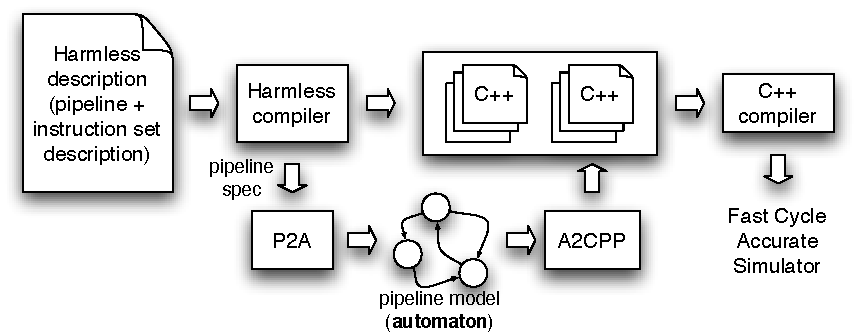
\includegraphics[width=0.8 \linewidth]{../common/images/devTools.pdf}
    \caption{Development chain}
    \label{fig:devTool}
  \end{center}
\end{figure}

These tools are:
\begin{itemize}
\item \gadl\ reads the file description in \harmless. This is the only tool necessary to generate a instruction set simulator (ISS);
\item  \texttt{p2a} and \texttt{a2cpp} are tools that are used for modeling the pipeline, when describing the internal architecture.  A description file of the pipeline is generated by \gadl\ according to the \h\ description,this is the input file of p2a. When the automaton has been generated by p2a, a second tool a2cpp translates the automaton description into $C++$ code, modeling of the pipeline.
\end{itemize}

This documentation focuses on the \gadl\ tool as the integration with the 2 other tools is in early stages of development.

\section{Building \gadl\ from sources}
The build process is made using a python script at the root of the archive : \texttt{buildHarmless.py}. Just configure your Internet access (proxy) if required and run the script. The build script:
\begin{itemize}
\item get the \texttt{galgas} compiler, as \gadl\ is written using the \texttt{galgas} language;
\item build the \texttt{p2a} and \texttt{a2cpp} tools;
\item build the library \texttt{libelf} that will be used to read .elf binary files for the simulators\footnote{\gadl\ is not compatible with the \texttt{libelf} library typically found on Linux distributions (including Ubuntu). Indeed, this library is linked to the simulator generated by \gadl, and we cannot impose a license to the generated code (That is the case with the GNU GPL. We use instead a library under the GNU LGPL. The library can be found on \url{http://www.mr511.de/software/english.html}}.
\end{itemize}

The script does not depends on specific tools (the only specific tools \texttt{galgas} is retrieved from Internet by the script). On Ubuntu/Debian systems, you should only install before basic development tools:
\texttt{apt-get install build-essential}


This script generates one big self-contained binary file that can generate a simulator from a description. The script is tested on Mac OS X, Linux x86/32 bits, Linux x86/64 bits and Linux ARMv6/32 bits. This has not been tested on Windows. 

Please report any problem during install to \url{mailto:harmless@irccyn.ec-nantes.fr}.

\subsection{Description editor}
A syntax file is provided for the \emph{Vim}\footnote{\url{http://www.vim.org}} editor, allowing syntax coloration. You only have to copy the syntax file to \texttt{~/.vim/syntax}. The directory have to be created if it does not yet exist.

With Mac OS X (10.5 required) an XCode project is provided. It can compile directly \gadl, but also build an application (Mac OS X bundle) to edit \harmless\ descriptions. It embeds a text editor with syntax highlighting and \gadl\ compiler.

\section{Dependencies for the simulator generation}

The generated simulator is written in $C++$  and can be used directly, without any dependency. However, a number of dependencies can be added to obtain additional services:
\begin{description}
\item[python] This allows to use the simulator in a Python script, and therefore does not require to recompile the simulator for each new scenario. The open source \texttt{swig}\footnote{\url{www.swig.org}} tool is used to generate the Python wrapper.
\item[libelf] This library allows to read \emph{elf} files, in addition to the default formats (SRecord Motorola and Intel Hex)
\end{description}

This section provides information on how to install these dependencies.

\subsection{Using the simulator with Python}
The simulator is generated in $C++$  and can be used in a Python script (version 2.5 and 2.6 tested). To enable the compilation of the Python wrapper, it is necessary to install the \texttt{Swig} tool:
\begin{itemize}
\item Linux Ubuntu: packages \texttt{swig} and \texttt{python2.5-dev}. The Python interpreter is installed by default.
\item Mac OS X: all is already included in the development tools (10.5).
\item MS Windows: Not tested.
\end{itemize}

\subsection{Library to read ELF files}
\label{sec:elf}
By default, \gadl\ can read the following file formats:
\begin{itemize}
\item Motorola SRecord (SREC)\footnote{\url{http://en.wikipedia.org/wiki/SREC_(file_format)}};
\item Intel Hex\footnote{\url{http://en.wikipedia.org/wiki/Intel_HEX}};
\end{itemize}
To add support for ELF format files \footnote{\url{http://en.wikipedia.org/wiki/Executable_and_Linkable_Format}}, an extra library is required. This last format has the advantage of encapsulating symbols (global variables, functions \ldots) in addition to executable code. 


\emph{Note}: \gadl\ is not compatible with the \texttt{libelf} library typically found on Linux distributions (including Ubuntu). Indeed, the library is linked to the simulator generated by \gadl, and it is not reasonable to impose the generated code to be under a license compatible with the GNU GPL\footnote{\url{http://fr.wikipedia.org/wiki/Licence\_publique\_generale\_GNU}}. We use a library under the GNU LGPL\footnote{\url{http://fr.wikipedia.org/wiki/Licence\_publique\_generale\_limitee\_GNU}}. The library can be found on \url{http://www.mr511.de/software/english.html}. To install it:
\begin{verbatim}
$ ./configure
$ make
$ sudo make install
\end{verbatim}

A local use is preferable on Linux distributions, to prevent conflicts with the other presents.

\emph{Note}: By default, the simulator is generated in 64-bit mode (compiler flag \texttt{-m64}), which gives much better simulation performance. In this case, the library libelf must also support 64-bit:
\begin{verbatim}
$ ./configure
$ make CFLAGS=-m64 LDFLAGS=-m64
$ sudo make install
\end{verbatim}

To stay in 32 bits, you should edit the generated \texttt{Makefile} and remove the \texttt{-m64} flag in \texttt{CFLAGS} and \texttt{LDFLAGS} (or better, update the Makefile.tpl in the template directory).



\section{Generation of a simulator}
The generation of the simulator is from the master file in the case of a description distributed over several files(voir section \ref{sec:plusieursFichiers}).

\gadl\ is a command line tool. Options availables are:
\begin{verbatim}
$ gadl --help
Compiled in 32 bits mode.
Usage : gadl [--help] [--version] [--lexical-analysis-only] [--parse-only] [-v] [--verbose] [--log-file-read] [--no-file-generation] [--Werror] [--detailled-error-messages] [-f] [--message-if-no-format] [-b] [--no-behavior] [-c] [--no-check] [-a] [--no-deasm] [-t] [--no-timing] [-s] [--speed] [-w] [--warn-trunc] [--max-errorss=number] [--max-warningss=number] [--model=string] [--templates=string] file...
Options:
 --help               Display help information
 --version            Display version
 --lexical-analysis-only
                      Perform only lexical analysis on input files
 --parse-only         Parse only input files
 -v,--verbose         Verbose Output
 --log-file-read      Log every file read
 --no-file-generation Do not generate any file
 --Werror             Treat warnings as errors
 --detailled-error-messages
                      Print detailled error messages
 -f,--message-if-no-format
                      get a message when an instruction signature found in a behavior or a syntax part have no corresponding format.
 -b,--no-behavior     does not take into account instruction behavior part. It is not possible to generate an instruction set simulator (ISS)
 -c,--no-check        Remove time consuming checks: orthogonality of instruction set.
 -a,--no-deasm        does not take into account instruction syntax part. It is not possible to generate a dissassembler
 -t,--no-timing       does not take into account instruction timing part. No cycle count. Simulation should be faster.
 -s,--speed           speed option. May be more difficult to debug. Inline component methods.
 -w,--warn-trunc      Warn if the result of an expression may be truncated
 --max-errors=number (default value : 0)
                      Stop after the given number of errors has been reached (by default: 100)
 --max-warnings=number (default value : 0)
                      Stop after the given number of warnings has been reached (by default: 100)
 --model=string       model name that will be generated. By default, all the model defined in the description file are generated.
 --templates=string   Template directory
Handled extension:
 .hadl                a gadl file that can be parsed with an LL1 grammar
\end{verbatim}

For each model described in the description, a directory is created containing the source code of the simulator. Consider for example the description file \texttt{avr.hadl} (included in \gadl\ sources) that contains the model \texttt{AT90CAN128}. The following command:

\begin{verbatim}
$ gadl ./avr.hadl
\end{verbatim}
create the directory  \texttt{./AT90CAN128}, which contains simulator sources. Most important files are:

\begin{verbatim}
Makefile           #file to generate the simulator (requires GNU Make)
arch.h             #main class of the simulator (arch)
arch.i             #C++/Python wrapper file (Swig)
format_all.dot     #describe the tree of the binary description of the instruction set (graphViz)
instConstruct.cpp  #instruction constructor (big file :-/)
instDecoder.cpp    #decode file (related to 'format')
instExec.cpp       #code executed by instructions (related to 'behavior')
instMnemo.cpp      #mnemonic of instructions (related to 'syntax')
instruction.h      #instruction classes
instruction.log    #debug information about the binary part
main.cpp           #simple scenario for the standalone simulator (not used with Python)
main_gdb.cpp       #simulate a gdb-server to use with GNU GDB (not used with Python)
storage.h          #memory model
types.h            #internal data types
\end{verbatim}

\subsection{Compilation options}
\label{sec:cflags}
Different compilation flags are available to modify the simulator behavior:
Main compilation parameters (\texttt{CFLAGS} in \emph{Makefile}) are:
\begin{description}
\item[HOST\_IS\_LITTLE\_ENDIAN] host is \emph{little endian}. This information is required by the \emph{storage} module.
\item[HOST\_IS\_BIG\_ENDIAN] host is \emph{little endian}. This information is required by the \emph{storage} module.
\item[INST\_DECODER\_CACHE\_STATS] This option allows to record memory instruction cache stats (nb of accesses, ratio hit/miss). The simulator speed is slightly altered.
\item[GADL\_NO\_ACTION] This option greatly accelerates the simulation speed. The \emph{action} are used to associate the execution of a piece of code to a memory access (read, write). Actions are used for peripherals description (\texttt{when} keyword). See section \ref{sec:whenReadWrite}.
\item[DEBUG\_MNEMO] To debug syntax part. the internal name of the instruction is printed with the mnemonic.
\item[DEBUG\_STORAGE\_ACCESS] To debug. Each memory access (read or write) is written on stdout. The simulator speed is altered
\item[DO\_NOT\_USE\_INTERNAL\_INSTRUCTION\_CACHE] To debug. Does not use the internal instruction cache associated to the decoder.
\item[DEBUG\_STORAGE\_ADDRESS\_RANGE] To debug. For each memory access, the simulator verifies that the address is in the correct range. Without this option, if an address is our of the memory chunk, a segfault should happen!
\end{description}

The \texttt{Makefile} should be used to generate the simulator (you should have a look to this documented file). Main targets are:
\begin{description}
\item[make standalone] generates a \emph{standalone} simulator. The simulation scenario is contained in the file \texttt{main.cpp};
\item[make python] generates a \emph{python library} of the simulator, see \ref{sec:python}. An example of how to use the python API is included with the AVR example.
\item[make gdb] generates a \emph{gdb server} simulator. This simulator can be used interactively used with gdb, using a UNIX socket. It has been tested successfully with Eclipse and the AVR module. This target works on POSIX hosts (Linux, Mac OS X).
\item[make clean] remove generated files.
\end{description}


\section{Using the simulator}
The API is available both for $C$/$C++$ and Python (through the SWIG wrapper).

The main $C++$ object is \texttt{arch} that should be used to have an instance of the processor.

Following sub-sections give main functions to deal with the simulator.
\subsection{System Observation}

\paragraph{\texttt{void decoderStats()}}
The method displays information on the internal decoder cache (used to speed up simulation). This command is valid only if the cache is used to decode (no option \texttt{DO\_NOT\_USE\_INTERNAL\_INSTRUCTION\_CACHE}) and if statistics are allowed (\texttt{INST\_DECODER\_CACHE\_STATS}), see section \ref{sec:cflags}:
\begin{verbatim}
Internal decoder instruction cache Ratio
    12128 accesses.
    Miss : 1217
    Hit : 10911
    Hit Ratio : 0.899654
    cache contains : 524 instructions
    (capacity is 1024 instructions)
    cache use ratio : 0.511719
\end{verbatim}

\paragraph{\texttt{unsigned int const getNBCycles()}} give the number of cycles since the beginning of the simulation. This is not used in the ISS mode (Instruction Set Simulation).
\paragraph{\texttt{unsigned int const getNBInstructions()}} give the number of instruction executed since the beginning of the simulation.
\paragraph{\texttt{string disassemble(const unsigned int ipStart, const int nbInst, bool verbose)}} disassemble code from address
\texttt{ipStart}, for \texttt{nbInst} instructions. If \texttt{verbose} is \texttt{true}, The decoding address and the instruction binary code are displayed.

\subsection{Execution}
\paragraph{\texttt{void reset()}}
At this date, it only reset the program counter.

\paragraph{\texttt{void execInst(const unsigned int nb)}} Execute \emph{a maximum of} \texttt{nb} instructions, either in CAS (Cycle Accurate Simulation) or ISS (Instruciton Set Simulation). If breakpoints are used, it should stop before.

\paragraph{\texttt{void runUntil(const unsigned int addr, const unsigned int max)}} simulate until the program counter is  \texttt{addr}. The simulator executes \emph{a maximum of} \texttt{max} instructions. If breakpoints are available, they are more efficient (no test at each clock cycle).

\paragraph{\texttt{bool readCodeFile(const char *filename, const bool verbose = false)}} read a binary code file and put it into the memory. Valid formats are: SRecord, Intel Hex or .elf, voir section \ref{sec:elf}). An error is generated if the file format is not recognized. Only memory section with \texttt{program} in the \h\ description of the memory can get program code (see section \ref{sec:mem_program}).

\subsubsection{Breakpoints}
Using breakpoints requires the \emph{actions} (execution of a piece of code related to a memory access (read, write or execute). Compilation flag \texttt{USE\_INTERACTIVE\_SIMULATION} should be set, and \texttt{GADL\_NO\_ACTION} should \emph{not} be set. see section \ref{sec:cflags}.
\paragraph{\texttt{void addBreakpoint(const unsigned int addr)}} Add a breakpoint for interactive simulation. An error is generated if there is already a breakpoint.
\paragraph{\texttt{void addBreakpoint(const char *symbolName)}} Add a breakpoint using the symbol name instead of the address (if symbols are available, with ELF files).
\paragraph{\texttt{void removeAllBreakpoints()}} 
\paragraph{\texttt{void removeBreakpoint(const unsigned int addr)}} Remove breakpoint at the specified address. An error is generated if there is not breakpoint.
\paragraph{\texttt{void removeBreakpoint(const char *symbolName)}} remove a breakpoint using symbol name instead of address.

\paragraph{\texttt{storage * getProgramChunk(const unsigned int address)}} Allow to get the memory chunk related to an address. This allows to read or write data in memory (see \texttt{storage.h} for further details).
\paragraph{\texttt{void setProgramCounter(u32 val)}} Define the value of the program counter (independently of the name used in the description (IP, PC,  \ldots).

\paragraph{\texttt{u32 programCounter()}} Read the value of the program counter (independently of the name used in the description (IP, PC,  \ldots).

\subsection{Symbols}
Using symbols instead of memory addresses is available only for .ELF files (see section \ref{sec:elf}).

\paragraph{\texttt{bool getSymbolObjectAddress(const char *symbolName, u32 \&v\_addr, u32 \&size)}} Search for the virtual address and size of the symbol name. It returns true if a symbol have been found, and updates \texttt{v\_addr} and \texttt{size}
\paragraph{\texttt{bool getFunctionName(const char *symbolName, u32 \&v\_addr)}} Search for the virtual address and size of the symbol name. It returns true if a symbol have been found, and updates \texttt{v\_addr}

\paragraph{\texttt{u32 getPhysicalAddress(const u32 v\_addr, bool \&found)}}  allows to get the physical address from the virtual one. \texttt{found} is set to \texttt{false} if the value is not in any available range.

it is easier to pool the common description of instructions

\subsection{Using Python}
\label{sec:python}
The main advantage of using Python to run scenarios is that it is no more necessary to recompile the simulator for each new scenario. When compiling the harmless simulator, a wrapper is generated with swig and a python module is built. In Python, it is then possible to call any C methods defined in the first part of this section.

For example, consider the AVR simulator provided in the examples directory. The model is called \texttt{AT90CAN128}, which is the name of the module to call. The following script calculates the number of instructions between 2 access to the function \texttt{function\_of\_task\_startTask}, 10 times:

\lstset{language=Python}
\begin{lstlisting}
#!/usr/bin/python
from AT90CAN128 import arch

f=arch()
f.readCodeFile("../trampoline.elf")
f.addBreakpoint("function_of_task_startTask")
nbInst = 0
f.printRegs()
for i in range(10):
    f.execInst(10000000) #run until breakpoint
    print f.getNBInstructions() - nbInst,  " insts between 2 breakpoints"
    nbInst = f.getNBInstructions()
f.printRegs()
f.decoderStats()
\end{lstlisting}
\lstset{language=Harmless}
